\title{Библиотека параллельной сборки мусора для С++}

\titlerunning{Библиотека параллельной сборки мусора для С++}

\author{Моисеенко Евгений Александрович}

\authorrunning{Е.А.Моисеенко}

\tocauthor{Е.А.Моисеенко}
\institute{Санкт-Петербургский государственный университет\\
\email{evg.moiseenko@mail.ru}}

\maketitle

\newcommand{\code}[1]{\textsf{#1}}

\begin{abstract}
В работе описывается алгоритм сборки мусора для языка C++, 
реализованный в виде библиотеки, не требующей поддержки со стороны компилятора. 
Реализованный сборщик мусора является 
\emph{точным}, т.е. способным точно идентифицировать указатели на управляемые объекты, 
\emph{инкрементальным}, 
\emph{копирующим}, т.е. способным улучшать локальность памяти за счёт перемещения объектов, 
\emph{потокобезопасным} и \emph{параллельным}. 
В работе также представлен обзор существующих решений задачи сборки мусора 
для языка C++, и проведена апробация результата.
\end{abstract}

\section*{Введение}

Синтаксический анализ, как правило, используется для построения структурного представления кода с использованием грамматики, описывающей разбираемый язык. Абстрактное синтаксическое дерево, являющееся результатом работы синтаксического анализатора, в дальнейшем используется для проведения статического анализа кода или же в каких-то других целях. Как правило, на вход синтаксическому анализатору подаётся линейная последовательность токенов, представляющая код программы. Однако могут возникать ситуации, когда вход не может быть представлен линейно. Такие ситуации могут возникать, например, при автоматической генерации кода. Генерация может происходить в циклах, с использованием условных операторов или строковых операций. Поэтому для описания генерируемых цепочек можно использовать конечный автомат, порождающий цепочки, который уже не будет являться линейным. Такую задачу будем называть синтаксическим анализом регулярных множеств.

Кроме этого, ещё одной областью, где может быть применим синтаксический анализ регулярных множеств, является бионформатика. Одной из часто возникающих задач в биоинформатике является классификация организмов, находящихся в образцах, полученных из окружающей среды~\cite{bioRNA}. По образцам строится метагеномная сборка, которая содержит в себе смесь из ДНК всех содержащихся в сборке организмов. В свою очередь ДНК является последовательностью символов в алфавите \{A, C, G, T\}. ДНК организмов, которые относятся к одному и тому же виду, содержат одинаковые подцепочки, которые и необходимо выделить, чтобы классифицировать организм. Как правило, эти подцепочки~--- это последовательности РНК. РНК может быть описана с помощью грамматики. Метагеномная сборка, в свою очередь, может быть представлена в виде графа с цепочками на рёбрах. Таким образом, в таком графе необходимо найти цепочки, выводимые в грамматике, описывающей РНК. 

Грамматики, описывающие структуру РНК, являются неоднозначными. Грамматика называется неоднозначной, если одна и та же цепочка может быть выведена несколькими способами. Такие алгоритмы синтаксического анализа как LR и LL не позволяют обрабатывать неоднозначные грамматики. Для работы с неоднозначными грамматиками существуют алгоритмы обобщённого синтаксического анализа GLR~\cite{GLR}, GLL~\cite{GLL}. В рамках проекта YaccConstructor~\cite{YaccConstructorPage, YaccConstructorPaper} был реализован алгоритм GLL, кроме того, была предложена его модификация для обработки нелинейных входных данных~--- графов. Реализованная модификация позволяет находить цепочки транспортной РНК (тРНК) в небольших метагеномных сборках, возвращая координаты начала и конца найденной цепочки. Проблема заключается в том, что грамматика для описания тРНК является сильно неоднозначной, что сказывается на производительности и точности полученных результатов. Для повышения точности можно применять конъюнктивные грамматики~\cite{ConjGrammars}, в которых для описания продукций используется операция конъюнкции. Такие грамматики расширяют класс контекстно-свободных языков и позволяют точнее описать структуру тРНК. Данная работа посвящена описанию модификаций решения на основе алгоритма GLL для работы с конъюнктивными грамматиками.

\section{Постановка задачи}

В данной работе были поставлены следующие задачи:

\begin{itemize}
\item проанализировать ограничения и недостатки текущей версии библиотеки сборки мусора;
\item предложить и реализовать новые методы для модернизации библиотеки;
\item реализовать и встроить в библиотеку алгоритм инкрементальной параллельной маркировки; 
\item протестировать функциональность и производительность новой версии библиотеки.
\end{itemize}

\section{Обзор}
\lstset{basicstyle=\normalsize\ttfamily, columns=fullflexible}
В данном обзоре рассматриваются некоторые подходы к заданию принтеров и форматеров, а также плагин Grammar-Kit для IntelliJ IDEA, позволяющий по БНФ-грамматике задавать синтаксический анализатор целевого языка.
Используемые плагином грамматики рассматриваются на примере грамматики языка While \cite{paper:nielson}.

\subsection{Подходы к заданию принтеров и форматеров}
Рассмотрим некоторые подходы к заданию принтеров и форматеров.
\subsubsection{Задание форматеров по описанию синтаксиса}%Язык описания синтаксиса}
Существуют различные подходы к заданию принтеров для целевого языка.
Один из них описан в \cite{paper:tbe}.
Авторы предлагают язык описания синтаксиса, по которому можно получить и синтаксический анализатор, и принтер для языка.
Описание синтаксиса состоит из правил, которые схожи с правилами формальных грамматик, но которые также задают и стиль форматирования для данной структуры языка.
Приведенное ниже правило вывода описывает основные арифметические выражения:
{
    \lstinputlisting{codes/tbeif.txt}
    %% =================================================
    %% ПРИМЕР ПОИНТЕРЕСНЕЕ
    %% непонятно, как задаются условия форматирования
    %% =================================================
}
\noindent
Первое преобразование определяет шаблон для выражений, состоящих из чисел.
Остальные преобразования задают шаблоны для операций сложения и вычитания.
Каждое из них состоит из двух меток \lstinline{<Exp>} для подстановки выражений, арифметического знака, а также двух пробелов вокруг этого знака.
Само правило явно задает способ, которым будут отформатированы арифметические выражения полученного языка.
%При дальнейшем форматировании программ на данном языке, арифметические выражения будут иметь вид, задаваемый правилом.
Вместо пробелов можно также указать табуляции и/или переносы строк.
Недостатком данного подхода является то, что правила форматирования задаются заранее, и, чтобы их изменить, необходимо менять описание синтаксиса языка.
Кроме того, каждое такое правило задает единственный вариант форматирования данной структуры.

%\subsubsection{}
Наиболее близкий к нашей работе метод описан в \cite{paper:asf-sdf}.
Принтер языка может быть получен по ASF+SDF описанию языка \cite{paper:klint}, что представляет собой контекстно-свободную грамматику.
При этом правила форматирования не указываются.
Недостатком данного подхода является то, что при генерации принтера задается базовый стиль форматирования, и, чтобы его изменить, необходимо редактировать сгенерированный код, тогда как подход с использованием синтаксических шаблонов позволяет пользователю декларативным образом настраивать принтер.

\subsubsection{Форматеры, встроенные в IDE}
Так же широко распространены форматеры, встроенные в IDE.
Они используют множество настроек для задания стиля форматирования (рис.~\ref{ov:settings}).
Среди них: тип и размер отступов, расположение фигурных скобок в C-подобных языках, политика переноса списочных выражений на новую строку и десятки других.
Набор этих настроек выбирается разработчиком форматера на основе его представлений о возможных стилях кодирования для целевого языка.
Такие форматеры обычно тесно интегрированы с IDE, имеют высокую скорость работы, и их выразительности, как правило, достаточно для задания необходимого стиля форматирования.
Однако для поддержки нового языка необходимо определить нужный набор настроек и вручную реализовать форматер.
В случае, если пользователю необходимо придерживаться стиля кодирования некоторой существующей кодовой базы, то ему нужно самостоятельно определить значения этих настроек.
Данный недостаток отсутствует в работе \cite{paper:sformatters}, где авторы предлагают инструмент, позволяющий получить некоторые настройки форматера из существующего программного кода.
Недостатком подхода является то, что число этих настроек невелико: система позволяет определять только стиль отступов, стили именования идентификаторов, необходимое количество комментариев.
Другой подход \cite{blog:genformat} предлагает использование генетического алгоритма 
%\footnote{\texttt{https://en.wikipedia.org/wiki/Genetic\textunderscore algorithm}} 
для поиска настроек форматера в исходном коде программ на языке C.

%и в работе\footnote{\texttt{https://blog.jetbrains.com/clion/2015/11/applying-genetic-algorithms-to-automatic-code-formatting/}}. 
%Они представляют собой способы автоматического вычленения настроек форматирования из программного кода.
\begin{figure}[t]
    \centering
    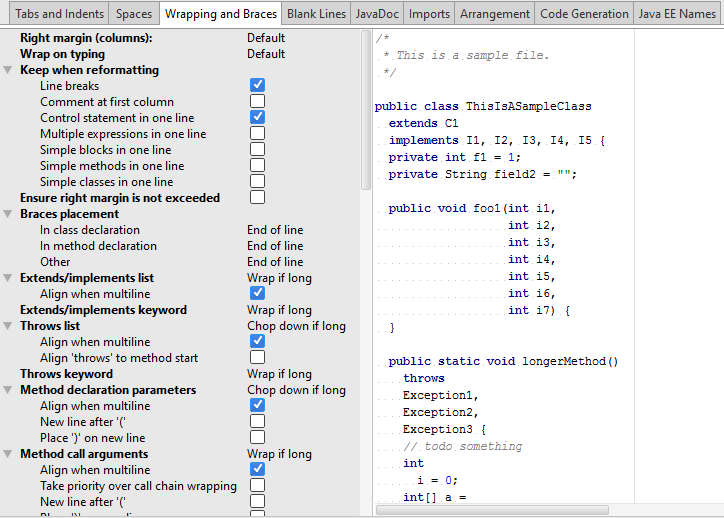
\includegraphics[width=.7\textwidth]{images/settingsjava.PNG}
    \caption{Настройки форматера языка Java в IntelliJ IDEA}
    \label{ov:settings}
\end{figure}

\subsection{Grammar-Kit}
Как уже было отмечено, для поддержки нового языка в платформе IntelliJ IDEA необходимо разработать синтаксический анализатор.
Для его генерации можно использовать плагин Grammar-Kit.
В качестве системы описания синтаксиса языка используется БНФ-грамматика.
Результатом работы плагина является код синтаксического анализатора и иерархия классов внутреннего представления. %(для IntelliJ IDEA~--- \emph{PSI-классов}).%PSI-классов.
%PSI-классом является каждая структура языка, вместе они образуют иерархию.

%Кроме того, при реализации поддержки нового языка в платформе возникает потребность в форматере.
%Мы хотим задавать принтер для языка, используя его грамматику.
% что тут еще описывать?
%\subsection{Грамматика языка While}
%Для апробации метода, описанного в \cite{paper:while}, использовался язык While, поэтому будем рассматривать грамматики, с которыми работает Grammar-Kit, на примере грамматики языка While.
Рассмотрим грамматику языка While, для которого производилась апробация метода, описанного в \cite{paper:while}.
%Рассмотрим БНФ-грамматику, использующуюся в плагине Grammar-Kit на примере грамматики языка While (рис.~\ref{ov:whileBnfFull}).
%\begin{figure}[p]
%\fvset{frame=lines,framesep=5pt}
While~--- язык программирования, содержащий следующие конструкции: чтение из стандартного потока (\lstinline{read}) и запись в стандартный поток (\lstinline{write}), оператор ветвления (\lstinline{if}), цикл с предусловием (\lstinline{while}); процедуры (\lstinline{proc}), бинарные выражения (\lstinline{binary_expr}), в том числе булевы (\lstinline{binary_bexpr}) и т. д.
% (рис.~\ref{ov:whileI},~\ref{ov:whileII},~\ref{ov:whileIII}).
\begin{figure}[h]
 %   \begin{pyglist}[numbers=left,numbersep=5pt]%, basicstyle=\ttfamily]
    \begin{lstlisting}[numbers=left, numbersep=3pt, basicstyle=\ttfamily\small, numberstyle=\tiny, frame=bottom, language={}]
whileFile  ::= proc_list stmt_list
stmt_list  ::= stmt*
proc_list  ::= procedure*
stmt       ::= skip|assign|if|while|write|read
skip       ::= 'skip' ';'
write      ::= 'write' '(' expr ')' ';'
read       ::= 'read' '(' id ')' ';'
assign     ::= id ':=' expr ';'
if         ::= 'if' '(' bexpr ')' 'then' stmt_list ('else' stmt_list)? 'fi'
while      ::= 'while' '(' bexpr ')' 'do' stmt_list 'od'
procedure  ::= 'proc' id '(' param_list ')' stmt_list 'endp'
param_list ::= ref_expr? (',' ref_expr)*
...
 \end{lstlisting}
    \caption{Грамматики языка While. Операторы языка}
    \label{ov:whileI}
\end{figure}
\noindent
На рис.~\ref{ov:whileI} представлена часть грамматики языка While, задающая множество операторов.
Рассмотрим правило грамматики, задающее оператор ветвления.
Правая часть правила состоит из терминалов \lstinline{'if'}, \lstinline{'then'} \lstinline{'('} и др.; нетерминалов: \lstinline{bexpr}, \lstinline{stmt_list}, а также условного вхождения \lstinline{('else' stmt_list)?} (то есть конструкция может отсутствовать в программах на данном языке).
Некоторые правила грамматики имеют модификаторы, которые используются для дополнительных указаний генератору синтаксического анализатора (рис.~\ref{ov:whileII}).
\begin{figure}[h]
    %\begin{pyglist}[numbers=left,numbersep=5pt]
    \begin{lstlisting}[numbers=left, numbersep=3pt, basicstyle=\ttfamily\small, numberstyle=\tiny, frame=bottom, language={}]
...
fake ar_op        ::= plus_op|mul_op
fake binary_expr  ::= expr ar_op expr 

expr              ::= factor plus_expr *
left plus_expr    ::= plus_op factor
plus_op           ::= '+'|'-'
private factor    ::= primary mul_expr *
left mul_expr     ::= mul_op primary
mul_op            ::= '*'|'/'|'%'
private primary   ::= literal_expr | ref_expr | paren_expr
paren_expr        ::= '(' expr ')'
ref_expr          ::= id
literal_expr      ::= number

fake bl_op        ::= or|and
fake binary_bexpr ::= bexpr bl_op bexpr
...
    \end{lstlisting}
    %\end{pyglist}
    \caption{Грамматика языка While. Выражения с модификаторами}%?
    \label{ov:whileII}
\end{figure}
\noindent
Модификатор \lstinline{fake} указывает системе, что не нужно генерировать код синтаксического анализатора для обработки данной структуры, однако генерируется иерархия классов внутреннего представления, \lstinline{private} указывает, что не будет сгенерирована иерархия классов, \lstinline{left} используется для поддержки левоассоциативности, а также некоторые другие\footnote{Посмотреть полный список можно по адресу \texttt{https://github.com/JetBrains/Grammar-Kit}}.
Модификатор \lstinline{private} используется для правил грамматики, которые не имеют представления в синтаксическом дереве.
Среди них те, которые используются для устранения левой рекурсии.
%которые не влияют на синтаксис языка, например, такие, которые используются для устранения левой рекурсии.
Например, на рис.~\ref{ov:whileExpr} представлено описание правил с рис.~\ref{ov:whileII} (строки 5--14), но в более естественной для человеческого восприятия леворекурсивной форме.
\begin{figure}[h]
    %\lstinputlisting{codes/whileExpr.txt}
    %\begin{pyglist}[numbers=left,numbersep=5pt]
    \begin{lstlisting}[numbers=left, numbersep=3pt, basicstyle=\ttfamily\small, numberstyle=\tiny, frame=bottom, language={}]
expr         ::= plus_expr | mul_expr | paren_expr | ref_expr | literal_expr
plus_expr    ::= expr plus_op expr
plus_op      ::= '+'|'-'
mul_expr     ::= expr mul_op expr
mul_op       ::= '*'|'/'|'%'
paren_expr   ::= '(' expr ')'
ref_expr     ::= id
literal_expr ::= number
    \end{lstlisting}
    %\end{pyglist}
    \caption{Грамматики языка While. Выражения в естественной леворекурсивной форме}
    \label{ov:whileExpr}
\end{figure}
\noindent
Однако грамматика, с которой работает Grammar-Kit, не должна содержать леворекурсивных правил.
Устраняя левую рекурсию, мы получим описание выражений на рис.~\ref{ov:whileII} (строки 5--14).
Кроме того, появляются новые правила, которые с точки зрения синтаксического анализа (а следовательно, и форматирования) являются избыточными.
В данном случае такими являются \lstinline{factor} и \lstinline{primary} на рис.~\ref{ov:whileII}.
\begin{figure}[b]
    %\begin{pyglist}
    \begin{lstlisting}[numbers=left, numbersep=3pt, basicstyle=\ttfamily\small, numberstyle=\tiny, frame=bottom, language={}]
{   parserClass="com.intellij.whileLang.parser.WhileParser"
    psiClassPrefix="Psi"
    psiImplClassSuffix="Impl"
    psiPackage="com.intellij.whileLang.psi.impl"
    tokens=[...]
    ...
}
...
    \end{lstlisting}
    %\end{pyglist}
    \caption{Заголовок файла с грамматикой}
    \label{ov:whileIII}
\end{figure}
% про left
Каждый файл с грамматикой языка содержит в себе заголовок, в котором описывается различная дополнительная информация: используемые в сгенерированных файлах классы, префиксы и суффиксы сгенерированных классов внутреннего представления, Java-пакеты, множество терминальных символов грамматики (\emph{tokens}) и др. (см рис.~\ref{ov:whileIII}).





\section{Реализация}

В данном разделе приводится описание выполненных модификаций библиотеки.


\subsection{Остановка мира}
\label{sec:stw}
В разделе \ref{sec:old_lib} были перечислены недостатки использовавшегося алгоритма 
остановки мутатора. 
Для их преодоления был предложен новый подход. 
Вместо расстановки безопасных точек в примитивах библиотеки предлагается помечать 
небезопасные участки кода, а другие участки считать безопасными. 
Преимущество данного подхода в том, что теперь мутатор может быть уведомлен об инициации 
сборки мусора в любой момент своей работы. 
Если в момент инициации сборки поток находится в небезопасном участке, то его приостановка 
откладывается до момента, когда он покинет этот участок. 
Заметим, что небезопасными являются только участки кода, выполняющие некоторые операции с 
глобальными структурами данных (корневым множеством, кучей, и т.д.) и расположеные в 
примитивах самой библиотеки.

Для реализации этого подхода необходимо иметь возможность уведомить поток об инициации 
сборки мусора в любой момент времени. 
После получения такого уведомления поток должен приостановить свою работу до момента, 
когда сборка будет окончена. 
Подобный функционал может быть реализован при помощи механизма сигналов операционной системы 
Linux и примитивов синхронизации, являющихся асинхронно-сигналобезопасными. 
Далее в данной главе будут рассмотрены сигналы и реализация механизма их временной блокировки, 
учитывающая специфику их использования в нашей библиотеке. 
Также будет описана реализация асинхронно-сигналобезопасных примитивов синхронизации. 
В последнем подразделе описан новый алгоритм ``остановки мира''. 


\subsubsection{Сигналы ОС Linux}
Сигналы в Linux --- один из механизмов межпроцессорного взаимодействия \cite{book:os_linux}. 
Linux поддерживает несколько типов сигналов, каждый из которых имеет уникальный идентификатор 
и мнемоническое имя. 
Сигнал может быть отправлен процессу либо ядром операционной системы, либо другим процессом 
с помощью системного вызова \code{kill}. 
При получении сигнала вызывается соответствующий обработчик сигнала. 
Для некоторых типов сигналов разрешается переопределять обработчик сигнала (при помощи 
системного вызова \code{sigaction}). 
Также имеется возможность временно заблокировать доставку сигналов определенного типа 
(системный вызов \code{sigprocmask}).

Библиотека \code{pthreads} позволяет отправлять сигналы конкретному потоку процесса с 
помощью системного вызова \code{pthread\_kill}, тем самым позволяя использовать сигналы 
для межпоточного взаимодействия.


\subsubsection{Блокирование сигналов}
В библиотеке \code{pthreads} имеется функция \code{pthread\_sigmask} аналогичная 
\code{sigprocmask}, но блокирующая доставку сигналов только данному потоку. 
Однако при каждом вызове \code{pthread\_sigmask} происходит переход в \emph{режим ядра} 
(\emph{kernel mode}), что вызывет длительные задержки. 
Временное блокирование доставки сигнала об инициации сборки мусора очень частая операция. 
Например, она необходима при каждой модификации корневого множества. 
Из-за её низкой скорости выполнения может пострадать производительность всего приложения, 
используещего сборку мусора. 

Для того, чтобы ускорить блокирование доставки сигнала инициации сборки мусора, был 
реализован механизм, учитывающий специфику задачи. 
Идея заключается в том, чтобы отследить попытку доставки сигнала потоку, выполнившему его 
блокирование, и отложить выполнение обработчика до момента разблокировки. 
В каждом потоке объявляются две локальные для потока (\code{thread\_local}) переменные 
\code{depth} и \code{pending\_flag}. \code{depth} отслеживает вложенность блокировок, 
\code{pending\_flag} инициализируется значением \code{false}. 
В обработчике сигнала сначала проверяется значение \code{depth}. 
Если оно не равно нулю, значит в текущий момент доставка сигнала заблокирована, 
выставляется \code{pending\_flag} и происходит выход из обработчика. 
Иначе происходит нормальное исполнение обработчика сигнала. 
Для того чтобы заблокировать доставку сигнала поток просто инкрементирует переменную 
\code{depth}. 
При разблокировании доставки сигнала значение \code{depth} декрементируется, и если оно 
становится равным нулю и при этом установлен флаг \code{pending\_flag}, вызывается код 
обработчика сигнала, но уже без дополнительных проверок. 
Код обработчика сигнала, блокирования и разблокированя доставки сигналов на C++ может быть 
найден в листинге \ref{code:siglock}.

В таблице \ref{table:siglock} приводится сравнение времени работы механизма блокирования 
сигналов с помощью функции \code{pthread\_sigmask} и механизма, предложенного в нашей работе. 
Измерялось суммарное время работы пары операций ~---~ блокирования и разблокирования сигнала. 
В таблице приведено среднее время работы операций $\bar{x}$ и стандартное отклонение $s$. 
Заметим, что ускорения удалось достичь за счёт того, что предложенный подход к блокированию 
сигналов является менее общим и учитывает специфику нашей задачи.

\begin{table}[h!]
\caption{Сравнение времени работы двух методов блокирования сигналов (среднее время $\bar{x}$ 
и стандартное отклонение $s$ указано в наносекундах)}
\label{table:siglock}
\begin{center}
\begin{tabular}{|l|c|c|}
\hline
                            & $\bar{x}$    & $s$       \\ \hline
pthread\_sigmask            & 143.661      & 6.741     \\ \hline
siglock/sigunlock           & 3.965        & 0.033     \\ \hline
\end{tabular}
\end{center}
\end{table}


\subsubsection{Асинхронно-сигналобезопасные примитивы синхронизации}
Стандарт POSIX\footnote{Стандарт POSIX описывает интерфейс для доступа к функциям 
операционной системы. 
Обеспечивает переносимость прикладных программ между ОС, поддерживающими POSIX. \\
\url{http://pubs.opengroup.org/onlinepubs/9699919799/}} 
накладывает жёсткие ограничения на код, работающий внутри обработчика сигнала. 
Обработчик сигнала должен быть асинхронно-сигналобезопасной функцией 
(async-signal safe function)\footnote{Определение асинхронно-сигналобезопасной функции 
может быть найдено по ссылке\\ \url{https://www.securecoding.cert.org/confluence/
display/c/BB.+Definitions\#BB.Definitions-asynchronous-safefunction}}. 

После получения сигнала об инициации сборки мусора поток должен приостановить свою работу 
до тех пор, пока он не получит уведомление об окончании сбоки. 
Код, выполняющий эту задачу, должен работать в контексте обработчика сигнала, так как иного 
способа уведомить поток о некотором событии в произвольный момент времени кроме использования 
сигналов нет. 
Так как никакие из примитивов синхронизации библиотеки \code{pthreads} не являются 
асинхронно-сигналобезопасными\footnote{Список async-signal safe функций ОС Linux может 
быть найден по ссылке\\ \url{http://pubs.opengroup.org/onlinepubs/9699919799/functions/
V2\_chap02.html\#tag\_15\_04\_03}}, 
необходимо использовать собственную реализацию примитивов синхронизации.

В нашей библиотеке было реализована два примитива: \code{signal\_safe\_barrier} и 
\code{signal\_safe\_event}. 

\begin{itemize}
\item 
    \code{signal\_safe\_barrier} имеет два метода:
    \begin{enumerate}
    \item 
        \code{notify()} для уведомления о том, что поток достиг некоторой точки в программе;
    \item 
        \code{wait(size\_t n)} для приостановки текущего потока до момента, когда \code{n} 
        других потоков достигнут барьера.
    \end{enumerate}
\item 
    \code{signal\_safe\_event} также определяет два метода:
    \begin{enumerate}
    \item 
        \code{notify(size\_t n)} для уведомления \code{n} потоков о наступлении события;
    \item 
        \code{wait()} для ожидания события.
    \end{enumerate}
\end{itemize}

Оба примитива реализованы с помощью одной и той же техники. 
Системные вызовы \code{read} и \code{write}, предназначенные для чтения и записи данных из 
потока ввода-ввывода, являются асинхронно-сигналобезопасными. 
Кроме того, \code{read} является блокирующим, то есть поток, вызвавший \code{read}, 
будет приостановлен, пока из потока не будет прочитано указанное количество байт. 
На основе этих двух системных вызовов, а также системного вызова \code{pipe}, 
открывающего безымянный двунаправленный поток ввода-ввывода, и построены наши примитивы. 

Оба примитива реализованы как классы. 
В конструкторе они открывают безымянный поток ввода-вывода. 
Метод \code{notify()} класса \code{signal\_safe\_barrier} записывает один байт в этот поток. 
Метод \code{wait(size\_t n)} читает из потока \code{n} байт. 
Аналогично для \code{signal\_safe\_event}, \code{notify(size\_t n)} записывает \code{n} байт 
в поток, а \code{wait()} читает из потока один байт.

\begin{figure}
\begin{lstlisting}[language={c++}, caption={Блокирование доставки сигналов}, label={code:siglock}, basicstyle=\small]
thread_local volatile sig_atomic_t depth = 0;
thread_local volatile sig_atomic_t pending_flag = false;

void check_gc_siglock(int signum) {
    if (depth > 0) {
        pending_flag = true;
        return;
    }
    gc_signal_handler();
}

void siglock() {
    if (depth == 0) {
        std::atomic_signal_fence();
        depth = 1;
        std::atomic_signal_fence();
    } else {
        depth++;
    }
}

void sigunlock() {
    if (depth == 1) {
        std::atomic_signal_fence();
        depth = 0;
        std::atomic_signal_fence();
        bool pending = pending_flag;
        pending_flag = false;
        if (pending) {
            gc_signal_handler();
        }
    } else {
        depth--;
    }
}
\end{lstlisting}
\end{figure}


\subsubsection{Алгоритм остановки мира}
Опишем теперь сам алгоритм ``остановки мира''. 
Рассмотрим отдельно часть, отвечающую за приостановку потока и выполняющуюся в 
обработчике сигнала, и часть, инициирующую сборку. 
В ходе выполнения обе части синхронизируют свою работу с помощью одного объекта класса 
\code{signal\_safe\_barrier} и одного объекта \code{signal\_safe\_event}. 
В обработчике сигнала поток сначала вызывает метод \code{notify()} барьера, чтобы 
уведомить поток, иницировавший ``остановку мира'', что он достиг обработчика. 
Затем вызывается метод \code{wait()} события. 
Когда сборка мусора окончится, поток, выполнявший сборку, возобновит работу остальных 
потоков, вызвав метод \code{notify(size\_t)} этого события. 
Затем в обработчике события будет вызван \code{notify()} барьера ещё раз, чтобы 
уведомить поток инициатор, что обработка сигнала завершена, и поток возвращается к 
нормальному исполнению. 
Для того, чтобы два потока одновременно не инициировали ``остановку мира'', код инициирования 
защищён мьютексом. 
Псевдокод иницирования ``остановки мира'' приведён в листинге \ref{code:stw}.

\begin{figure}[h!]
\begin{lstlisting}[caption={Остановка мира},label={code:stw}]
lock(gc_mutex)
for (thread in threads)
    send(gc_signal, thread)
signal_safe_barrier.wait(threads.count - 1)
gc()
signal_safe_event.notify(threads.count - 1)
signal_safe_barrier.wait(threads.count - 1)
unlock(gc_mutex)
\end{lstlisting}
\end{figure}


\subsection{Закрепление объектов}
Механизм закрепления объектов, использовавшийся в предыдущей версии библиотеки 
(раздел \ref{sec:old_lib}), включал процедуру консервативного обхода стека потоков. 
Поэтому в некоторых ситуациях сборщик мог ошибочно не идентифицировать мусор. 
В новой версии реализован механизм закрепления объектов, лишённый этого недостатка, и 
кроме того, точно отслеживающий время, когда закрепление может быть снято.

Используется идиома RAII, упомянутая в разделе \ref{sec:cpp_solutions}. 
Вводится новый примитив ~---~ шаблонный класс \code{gc\_pin<T>}. 
Конструктор класса \code{gc\_pin<T>} принимает в качестве аргумента ссылку на объект типа 
\code{gc\_ptr<T>} и выполняет закрепление объекта, на который указывает этот \code{gc\_ptr}. 
В деструкторе \code{gc\_pin<T>} закрепление объекта снимается. 
Указатели на все закрепленные объекты хранятся в структуре данных, аналогичной той, 
что используется для хранения корневого множества (раздел \ref{sec:old_lib}). 
То есть используется список указателей, причём новые указатели вставляются в голову и 
при удалении список просматривается с головы. 
Также как и в случае корневого множества, каждый поток имеет собственный экземпляр списка 
закрепленных объектов. 
Таким образом, в конструкторе \code{gc\_pin<T>} указатель на объект вносится в список 
закрепленных объектов, а в деструкторе удаляется из него.

На этапе сжатия/освобождения кучи, после ``остановки мира'', сборщик просматривает списки 
закрепленных объектов всех потоков. 
У объектов из этих списков выставляется бит закрепления (наличие этого бита говорит сборщику 
о запрете перемещать данный объект), также они сканируются сборщиком (для того, чтобы 
пометить все объекты, достижимые из закрепленного, и предотвратить их удаление). 

Как уже упоминалось, закрепление объектов необходимо в двух случаях:
\begin{enumerate}
\item 
    Для передачи сырого указателя на управляемый объект в функцию, принимающую ``сырой'' 
    указатель как аргумент.
\item 
    Для закрепления указателя \code{this} при вызове оператора доступа к члену класса 
    (\code{operator->()}).
\end{enumerate}

В первом случае пользователь может самостоятельно создать объект типа \code{gc\_pin} и 
получить сырой указатель с помощью метода \code{get()} этого объекта. 
Стоит однако отметить, что время жизни полученного таким образом сырого указателя не 
должно превышать время жизни соответствующего объекта \code{gc\_pin}. 
Во втором случае объект \code{gc\_pin} создаётся неявно самой библиотекой. 
Используется следующее соглашения языка C++ 
\footnote{Working Draft, Standard for Programming Language C++,\\
\url{http://www.open-std.org/jtc1/sc22/wg21/docs/papers/2014/n4296.}\\{pdf}}
: если оператор доступа к 
члену класса (\code{operator->()}) возвращает объект типа, отличного от \code{T*}, 
вызывается оператор доступа к члену класса этого объекта. 
То есть, перегруженный оператор доступа к члену класса \code{gc\_ptr} создаёт на стеке 
объект типа \code{gc\_pin} и возвращает его, затем, согласно соглашению языка C++, 
вызывается оператор доступа к члену класса этого временного объекта, который уже возвращает 
сырой указатель. 
После этого вызывается деструктор временного объекта \code{gc\_pin}.  


\subsection{Инкрементальная параллельная маркировка}
Рассмотрим реализацию алгоритма инкрементальной параллельной маркировки, разработанную в 
рамках данной работы и внедренную в библиотеку точной сборки мусора для языка C++.

В нашей работе в фазе маркировки работа мутатора не приостанавливается, сборщик мусора 
работает параллельно с потоками мутатора. 
``Остановка мира'' происходит два раза за цикл сборки мусора: перед запуском этапа 
маркировки для сканирования корневого множества и для освобождения памяти после 
окончания маркировки. 
Выполнять маркировку параллельно могут сразу несколько потоков. 
Фаза маркировки начинается когда размер кучи достигает некоторого порогового значения. 

Для распределения работы между потоками-маркировщиками используется механизм 
\emph{пакетов работы} (\emph{work packet}), подобный описанному в статье 
\cite{barabash2005parallel}. 
Пакет представляет собой массив фиксированного размера, который содержит указатели на 
объекты, ожидающие сканирования. 
Сборщик мусора поддерживает глобальный пул пакетов. 
Каждый поток-маркировщик использует два пакета ~---~ входной (input) и выходной (output). 
Маркировщик по очереди вынимает указатели из входного пакета и сканирует объекты, на которые 
они указывают. 
Если обнаружится, что объект содержит указатели на другие объекты, они заносятся в выходной 
пакет. 
Когда входной пакет оказывается пуст или выходной пакет заполнен, маркировщик возвращает пакет 
в глобальный пул и получает новый пакет. 

Глобальный пул пакетов поддерживает три списка ~---~ список пустых пакетов, 
список частично (менее чем на 50\%) заполненных пакетов и список почти полностью 
(более чем на 50\%) заполненных пакетов. 
Каждый список также содержит мьютекс, для того чтобы синхронизировать операции добавления 
и удаления элементов при обращении нескольких потоков. 
Суммарное количество пакетов фиксированно, память для пакетов выделяется один раз 
при инициализации сборщика мусора. 
Когда поток-маркировщик запрашивает входной пакет у пула, выбирается пакет из почти 
полностью заполненных, а если таковых нет ~---~ из частично заполненных. 
При запросе выходного пакета возвращается пустой пакет, если же список пустых пакетов пуст, 
то пакет из частично заполненных. 
Изначально все пакеты находятся в списке пустых пакетов. 
При сканированни корневого множества сборщик запрашивает у пула необходимое количество 
выходных пакетов, копирует в них указатели на корневые объекты и возвращает пакеты в пул. 
После этого потоки-маркировщики начинают запрашивать входные пакеты и сканировать их. 

Использование механизма пакетов позволяет достаточно просто определить момент окончания 
фазы маркировки ~---~ когда количество пустых пакетов становится равным общему количеству 
пакетов фаза маркировки считается законченной. 

Рассмотрим также реализацию барьера записи. 
В нашей библиотеке барьер записи реализован программно и вызывается из конструктора 
копирования и оператора присваивания \code{gc\_ptr}. 
Барьер записи перехватывает операции записи только если сборщик находится в фазе маркировки. 
Мы используем барьер записи Дейкстры, его псевдокод приведён в листинге 
\ref{code:write_barrier}. 
Напомним, что барьер записи Дейкстры ``перекрашивает'' объект, ссылка на который записывается, 
в ``серый'' цвет, если раньше его цвет был ``белым''. 
Для этого каждый поток мутатора запрашивает у глобального пула пакетов один выходной пакет 
и помещает в него ссылки на ``перекрашенные'' в серый объекты. 
Когда пакет заполняется, поток возвращает его в пул и запрашивает новый. 
Заметим, что после окончания фазы маркировки у потоков мутатора могут остаться частично 
заполненные пакеты серых объектов. 
Данные пакеты сканируются уже после ``остановки мира''. 
Ожидается, что количество объектов в этих частично заполненных пакетах будет небольшим.

Также стоит отметить, что в фазе маркировки новые объекты создаются ``чёрными'', 
то есть гарантированно переживают текущий цикл сборки мусора.

Операции присваивания указателей и создания новых объектов очень часты, 
поэтому необходимо, чтобы проверка текущей фазы была достаточно быстрой. 
В нашей реализации для этого используется переменная \code{phase} типа 
перечисления (допустимые значения: \code{IDLE}, \code{MARKING}, \code{COMPACTING}). 
Изменения значения переменной \code{phase} происходят только во время остановок мира, 
а операции присваивания указателей и создания нового объекта помечены как ``небезопасные'', 
то есть во время их выполнения не может произойти ``остановки мира'' и, следовательно, 
не может измениться фаза сборки мусора.


\subsection{Параллельное сжатие}
В процедуру сжатия кучи также были внесены изменения с целью её распараллеливания. 
Как уже упоминалось в разделе \ref{sec:heap}, куча для объектов маленьких размеров 
представляет собой набор пулов, каждый из которых обслуживает объекты определенного размера. 
Ясно, что каждый пул можно сжимать независимо от остальных в отдельном потоке. 
В нашей реализации множество пулов разбивается на $n$ равных частей, 
где $n$ - количество доступных на данной системе ядер процессора, 
полученное с помощью функции из стандартной библиотеки 
\code{std::thread::hardware\_concurrency}. 
Затем создаётся $n$ потоков, каждый из которых поочередно сжимает пулы из 
соответствующей части с помощью двухпальцевого алгоритма \ref{sec:two-finger-compact}. 
Преимущество подобного статического разбиения работ в том, что потокам нет необходимости 
синхронизировать свою работу. 
С другой стороны, если окажется, что объекты распределены по пулам неравномерно, 
то сборщик не сможет полностью задействовать аппаратный параллелизм, так как некторые 
потоки закончат свою работу намного раньше остальных. 

Объекты большого размера выделяются с помощью системного вызова \code{mmap} и 
сохраняются в список больших объектов. 
Для таких объектов сжатие не выполняется. 
Память из-под объектов, объявленных сборщиком недоступными, возвращается операционной 
системе с помощью системного вызова \code{munmap}.
\section{Апробация}

Функциональность сборщика мусора была протестирована на модульных тестах, 
написанных вручную с помощью фреймворка \textbf{googletest}
\footnote{Google Test, Google's C++ test framework,\\ 
\url{https://github.com/google/googletest}}. 
Также было произведено тестирование производительности реализованного алгоритма 
инкрементальной параллельной маркировки. 
Для этой цели использовался известный тест Бёма, активно работающий с динамической памятью. 
В этом тесте строятся двоичные деревья различной глубины с различным количеством узлов. 
Деревья строятся двумя способами: от листов к корню и наоборот, от корня к листьям. 
Было выполнено сравнение библиотеки с аналогами, в частности, с ручным управлением памятью 
с помощью \code{new}/\code{delete}, с классом умного указателя \code{std::shared\_ptr}, 
реализующим подсчёт ссылок, а также с консервативным сборщиком мусора Бёма-Демерса-Вайзера 
c включенной и выключенной опцией инкрементальной маркировки. 
Наша библиотека тестировалась с четырьмя стратегиями: включенной/выключенной 
инкрементальной маркировкой и включенным/выключенным сжатием кучи. 

Измерялось суммарное время работы теста (рис.\ref{fig:boehm}), количество сборок мусора 
(на графике показано как целое число над соответствующим столбцом) и среднее время 
``остановки мира''(рис.\ref{fig:boehm_pause}). 
Все измерения были взяты как среднее и стандартное отклонение по 20 запускам теста. 
Хотя суммарное время работы сборщика с инкрементальной параллельной маркировкой и увеличилось, 
среднее время паузы существенно уменьшились. 
В частности, среднее время паузы при отключенном сжатии при инкрементальной маркировке примерно 
в шесть раз меньше, чем без неё. 
При одновременном включении и сжатия, и инкрементальной маркировки время работы теста 
существенно увеличивается. 
Это объясняется тем, что при инкрементальной маркировки доля объектов, переживающих текущий 
цикл сборки, больше, а время работы текущей реализации процедуры сжатия существенно 
увеличивается при увелечении размера кучи. 
Стоит отметить, что наша библиотека работает примерно в 4 раза медленее чем другие решения, 
участвовавшие в эксперименте, что свидетельствует о необходимости дальнейшей оптимизации.

\begin{figure}[ht!]
\centering
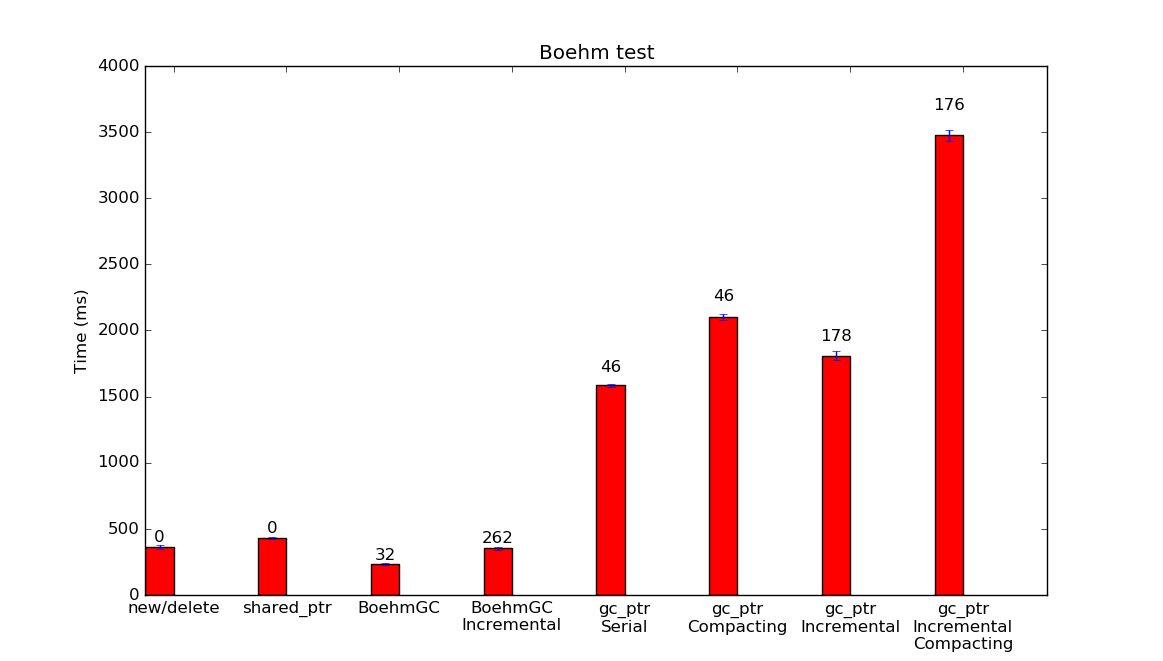
\includegraphics[width=\textwidth]{Moiseenko/images/boehm_all.png}
\caption{Тест Бёма. Суммарное время работы.}
\label{fig:boehm}
\end{figure}

\begin{figure}[h!]
\centering
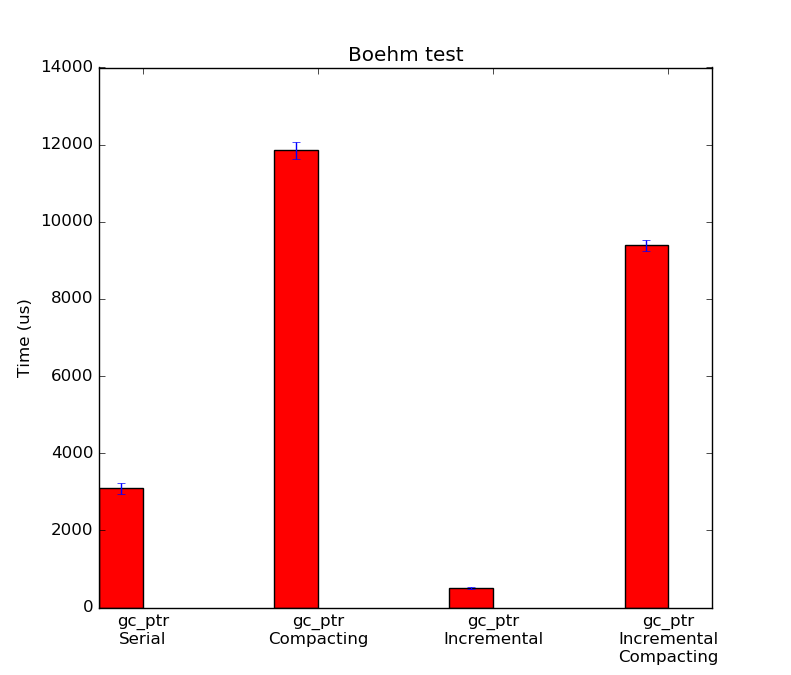
\includegraphics[width=0.8\textwidth]{Moiseenko/images/boehm_pause_all.png}
\caption{Тест Бёма. Среднее время паузы.}
\label{fig:boehm_pause}
\end{figure}

\begin{figure}[h!]
\centering
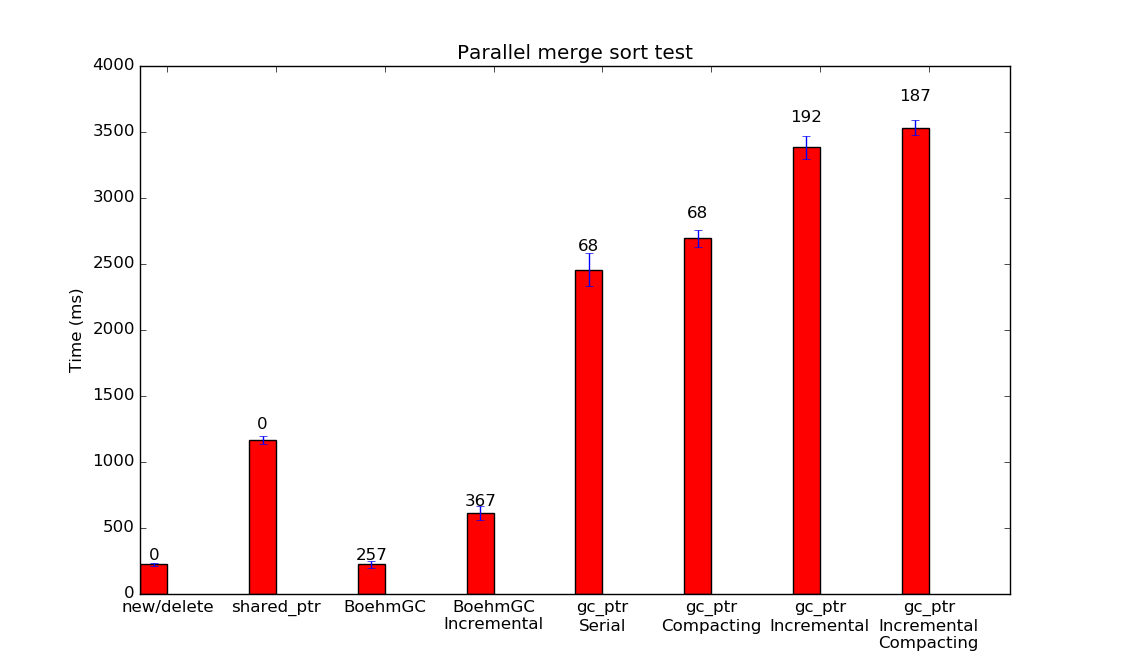
\includegraphics[width=0.8\textwidth]{Moiseenko/images/merge_sort_all.png}
\caption{Многопоточная сортировка слиянием. Суммарное время работы.}
\label{fig:merge_sort}
\end{figure}

\begin{figure}[ht!]
\centering
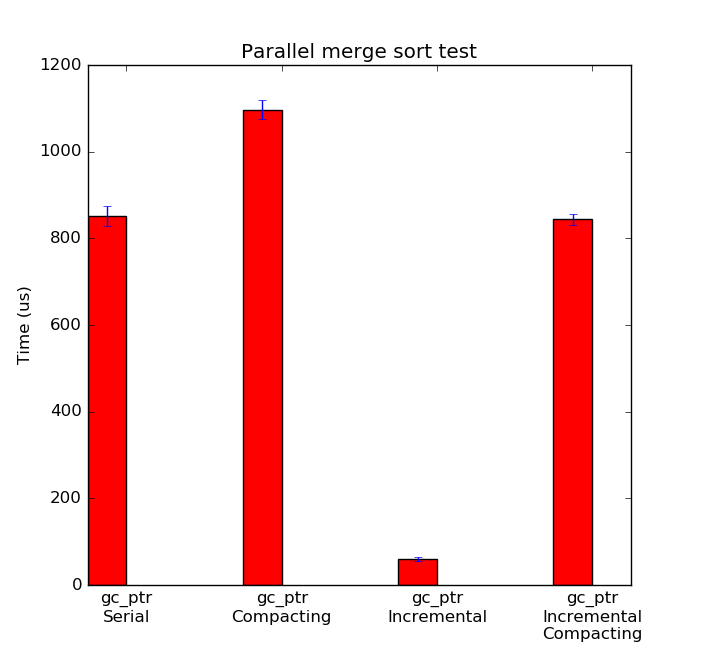
\includegraphics[width=0.7\textwidth]{Moiseenko/images/merge_sort_pause_all.png}
\caption{Многопоточная сортировка слиянием. Среднее время паузы.}
\label{fig:merge_sort_pause}
\end{figure}

Также было протестирована работа сборщика с многопоточным приложением. 
Для этой цели был написан тест, использующий алгоритм сортировки слиянием. 
В этом тесте генерируются односвязные списки. 
Каждый узел списка содержит одно случайное значение типа \code{int}. 
Список разделяется на несколько частей (по числу доступных ядер процессора), 
каждая часть сортируется в отдельном потоке сортировкой слиянием, 
затем части сливаются в единый список. 
Результаты замеров работы библиотеки, а также аналогов, на этом тесте представлены 
на рис.\ref{fig:merge_sort} и рис.\ref{fig:merge_sort_pause}. 
Видно, что результаты данного теста в целом повторяют результаты теста Бёма. 
\section*{Результаты}

В ходе работы были достигнуты следующие результаты:

\begin{itemize}
\item проанализированы ограничения и недостатки предыдущей версии библиотеки;
\item реализован новый алгоритм остановки мира; 
\item реализован новый алгоритм закрепления объектов;
\item реализована модификация алгоритма инкрементальной параллельной маркировки;
\item выполнена апробация: протестирована функциональность библиотеки, измерена её производительность, произведено сравнение с аналогами.
\end{itemize}


\begin{thebibliography}{99}

\bibitem{book:precisegc_secr}
    D. Berezun, D. Boulytchev.
    Precise Garbage Collection for C++ with a Non-cooperative Compiler.
    Proceedings of the 10th Central and Eastern European Software Engineering Conference 
    in Russia, 2014.

\bibitem{book:precisegc_berezun}
    Д. Березун.
    Реализация основных примитивов библиотеки неконсервативной сборки мусора для C++.
    Труды лаборатории языковых инструментов JetBrains, выпуск 2, 2014.

\bibitem{book:precisegc_samofalov}
    А.Самофалов.
    Библиотека почти точной копирующей сборки мусора для C++.
    Труды лаборатории языковых инструментов JetBrains, выпуск 3, 2015

\bibitem{book:jones1996garbage}
    Jones, Richard and Lins, Rafael D.
    Garbage collection: algorithms for automatic dynamic memory management.
    Wiley, 1996.

\bibitem{book:jones2011garbage}
    Jones, Richard and Hosking, Antony and Moss, Eliot.
    The garbage collection handbook: the art of automatic memory management.
    Chapman \& Hall/CRC, 2011.

\bibitem{dijkstra1978fly}
    Dijkstra, Edsger W and Lamport, Leslie and Martin, Alain J and Scholten, Carel S and 
    Steffens, Elisabeth FM.
    On-the-fly garbage collection: An exercise in cooperation.
    Communications of the ACM, vol. 21, num. 11, pp. 996---975, 1978.

\bibitem{boehm2007transparent}
    Boehm, Hans-J and Spertus, Michael.
    Transparent Programmer-Directed Garbage Collection for C+.
    URL: http://www.open-std.org/jtc1/sc22/wg21/docs/papers,
    num. 2310, 2007.

\bibitem{book:os_linux}
    А.М. Робачевский.
    Операционная система UNIX, 2 изд.,
    БХВ-Петербург, 2010.

\bibitem{boehm1993space}
    Boehm, Hans-Juergen. 
    Space efficient conservative garbage collection.
    ACM SIGPLAN Notices, vol. 28, num. 6, pp. 197--206,
    1993.

\bibitem{book:cpp_concurrency}
    Э. Уильямс.
    Параллельное программирование на C++ в действии. Практика разработки многопоточных программ.
    Litres, 2014.

\bibitem{barabash2005parallel}
    Barabash, Katherine and Ben-Yitzhak, Ori and Goft, Irit and Kolodner, Elliot K and 
    Leikehman, Victor and Ossia, Yoav and Owshanko, Avi and Petrank, Erez.
    A parallel, incremental, mostly concurrent garbage collector for servers,
    ACM Transactions on Programming Languages and Systems (TOPLAS),  vol. 27,
    num. 6, pp. 1097--1146, 2005.

\end{thebibliography}
